% !TeX document-id = {adfd8c77-9aa9-43e7-acaa-af378587f0c7}
% !TeX TXS-program:compile = txs:///pdflatex/[--shell-escape]
\documentclass{article}

\usepackage[utf8]{inputenc}
\usepackage[T1]{fontenc}
\usepackage{color}
\usepackage{soul}
\usepackage{amsmath}
\usepackage{amssymb}
\usepackage{listings}
\usepackage{minted}
\usepackage{hyperref}
\usepackage{graphicx}
\usepackage{calc}
\usepackage{enumitem}
\usepackage{standalone}

\usepackage{tikz}
\usetikzlibrary{datavisualization}
\usetikzlibrary{datavisualization.formats.functions}

\graphicspath{{img/}}
\setlength{\parindent}{0pt}

\begin{document}

\title{CW 19 summary}
\author{Alexander Pastor}
\date{08.05.2017}
\maketitle
\tableofcontents
\newpage

\section{Understanding RF Specifications}

\subsection{Basic Terminology}

\emph{digitizer amplitude error}

The following formula provides the dampening or attenuation factor E of the digitizer:

\begin{equation}
	E = 1- \frac{R}{\sqrt{1+R^2}}
\end{equation}

\medskip

A X-Hz digitizer is defined to have $ E = \frac{1}{\sqrt{2}}$ at the frequency X, which implies $R=1$ for the frequency X. X is called bandwidth of the digitizer in this context, and R is the ratio of the digitizer bandwidth and the maximum frequency of interest $\frac{f_d}{f_i}$.

\begin{figure}[h]
	\centering
	\label{amplitude_error}
	\documentclass[border=2mm,tikz]{standalone}
\usepackage{tikz}
\usetikzlibrary{datavisualization}
\usetikzlibrary{datavisualization.formats.functions}
\begin{document}
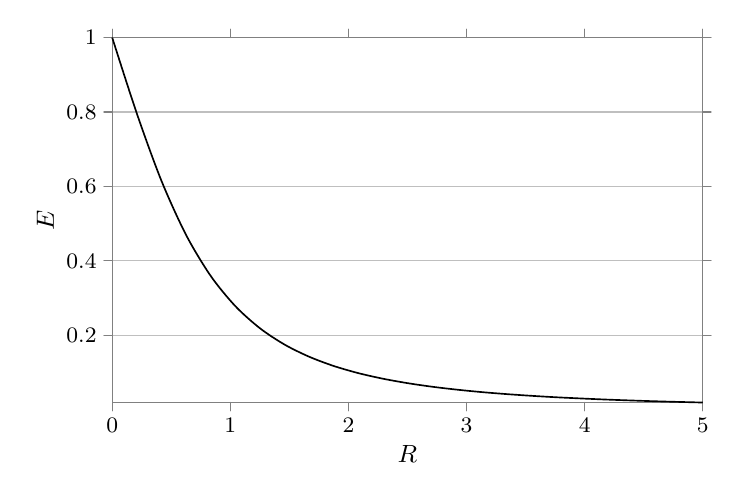
\begin{tikzpicture}
\datavisualization [scientific axes,
					y axis=grid,
                    y axis={label={$E$}},
                    x axis={label={$R$}},
                    visualize as smooth line,
                    scale = 1.5
                   ]

data [format=function]
{
  var x : interval [0:5];
  func y = 1 - ((\value x)/(sqrt(1 + \value x * \value x)));
};
\end{tikzpicture}
\end{document}
	\caption{Digitization error verus bandwidth ratio}
\end{figure}

It is recommended by NI to have X be 3 to 5 times higher than the frequency of interest. This corresponds to errors or dampening between 1.94\% and 5.13\% 

\bigskip

\emph{rise time}

Rise time is defined as the time a signal needs to rise from 10\% to 90\% of its steady-state or periodic maximum.

\bigskip

\begin{itemize}
	\item The rise time of a simple RC-circuit is about $\frac{0.35}{RC}$.
	\item The formula to calculate the total rise time of a digitized signal is: $$ T_{r_t} = \sqrt{{T_{r_s}}^2 + {T_{r_d}}^2}$$
	\item In order to minimize rise time errors NI recommends to have $T_{r_d}$ be around $\frac{1}{3}$ and $\frac{1}{5}$ of $T_{r_s}$.
\end{itemize}

\emph{Nyquist Theorem}

The bandwidth of the digitizer must be at least 2 times the maximum frequency of the signal to avoid aliasing. 

\medskip

$\Leftrightarrow$ To extinguish aliasing in the passband one either has to make sure the Nyquist Theorem is matched or apply a lowpass filter to limit the signal's bandwidth.

\bigskip

\emph{phase noise}

Phase noise is the frequency domain representation of time domain jitter. Jitter in turn is the first derivative of a delay. Phase noise is usually close to the carrier and thus measured in dBc (decibels relative to the carrier).

\bigskip

\emph{spectral density}

Measures the power per frequency in a frequency domain [W/Hz].

\bigskip

\emph{resolution bandwidth}

The resolution bandwidth equals the FFT bin size and is smallest resolvable frequency. It is inversely proportional to the number of samples.

\bigskip

\emph{noise density}

Noise level below which signal cannot be detected. One has to distinguish between broadband noise density of a sinusoidal and random (perhaps AWGN) noise. In the latter case one can use a narrow band filter to improve our signal. 

\bigskip

\emph{dynamic range}

Ratio between the highest and lowest signal level a circuit can take. Spurious dynamic range is the ratio between the highest and lowest signal level, without any unwanted sinusoidal frequencies. It is usually expressed in dB.

\bigskip

\emph{voltage standing wave ratio (VSWR)}

The VSWR is the reflected-to-transmitted wave ratio. Self-evidently, the smaller, the better.

$$
	VSWR = \frac{1+p}{1-p}
$$

where p is the reflection coefficient.

\medskip

Note that is also possible to represent reflections as return loss (in dB):

\begin{align*}
	RL \quad 	&= 10 	\log\left(\frac{P_\text{in}}{P_\text{reflected}}\right) 	\\
				&= 20 	\log\left(\frac{V_\text{in}}{V_\text{reflected}}\right) 	\\
				&= -20 	\log\left(\frac{V_\text{reflected}}{V_\text{in}}\right) 	\\
				&= -20 	\log\left(\lvert p \rvert\right)
\end{align*}
	


\bigskip

\emph{frequency response}

Just as a reminder: the frequency response is the fourier transform of the impulse response $h(t)$.

$$
	H(f) = \int_{-\infty}^{\infty} h(\tau) \cdot \exp(-j2\pi ft) \,d\tau
$$

\bigskip
 
\emph{modulation error ratio (MER)}

A measure of SNR for digitally modulated signals, also expressed in dB.

$$
	MER = \frac{\sum_{j=1}^{N} \tilde{I_j^2}+\tilde{Q_j^2}}{\sum_{j=1}^{N} (\tilde{I_j}-I_j)^2+(\tilde{Q_j}-Q_j)^2}
$$

Where the components with $\sim$ are the ideal and those without are the actually received components of the N symbols of the signal.

\bigskip

\emph{IQ procedure}

In-phase and quadrature demodulation procedure. 

\bigskip

\emph{error vector magnitude (EVM)}

Quantifies demodulation performance under the influence of noise. The EVM is the normalized root-mean-square of the difference of ideal and measured location over all symbols. It is normalized by the maximum length of an ideal symbol to make the EVM's value comparable under different system gain conditions.

$$
	EVM = \frac{\sqrt{\frac{1}{N}\sum_{j=1}^{N} (\tilde{I_j}-I_j)^2+(\tilde{Q_j}-Q_j)^2 }}{\lvert v_\text{max} \rvert}
$$

\bigskip

\emph{third-order intercept (TOI)}

Theoretical number. TOI is the power level when the third-order harmonic distortion has the same power level as the fundamental tone. The bigger the TOI, the better since it is a measure for the maximum RF-circuit power.

\section{Physical Layer Challenge}

\subsection{Basic Terminology}

\subsubsection{FIR Filters}

\emph{passband, transitionband, stopband}

The passband is the frequency band that is not attenuated band of a filter, i.e. that band of allowed frequencies. The stopband is the band that a filter stops, or attenuates strong enough, so that the signal amplitude for those frequencies is below the stopband threshold. The transitionband is an attenuated band between passband and stopband.  

\bigskip

\emph{filter tap}

A filter tap is a (coefficient, delay) pair. The number of taps is often denoted as N. This number is a good mesaure for the amount of filtering, the required space and the amount of calculation required by the filter. 

\subsubsection{Frame Synchronization}

\emph{frame preamble and start frame delimiter (SFD)}

Aliases: syncword or sync sequence framing.

Repetitive pattern of all the same nibbles (and thus bytes). Marks an Ethernet frame beginning. After the preamble the one-byte \emph{start frame delimiter} is located to mark the beginning of real data. This mechanism is employed to achieve a self-clocking protocol. The preamble is needed to resynchronize the receiver once a bit slip occurs.

\bigskip

\emph{CRC-based framing}

\color{blue}
[question] CRC-based framing is used in ATM protocols by reusing the header CRC. How exactly does this work? Also, I wondered since 802.11 and Ethernet both also have a FCS (CRC) at the end of their frames, do they use some kind of CRC-based / syncword-based framing at the same time? As of now I think it is as follows: 802.11 and Ethernet frame synchronization is syncword-based and CRC is employed for error correction only.
\color{black}

\bigskip

\emph{self-clocking signal}

Signal that is synchronized without a separate clock signal. Receiver synchronization information is contained in the signal (preamble+SFD).

\bigskip

\emph{bit slip}

A lost bit or an extra bit in the signal.

\bigskip

\color{blue}
[question] Why aren't Ethernet (and 802.11) using byte- or bitstuffing methods for frame synchronization? I thought maybe bit errors could corrupt the whole "synchronization complex", but one lost frame shouldn't be too bad? I guess that a big 56-bit preamble and 8-bit SFD might just be more robust against bit errors?
\color{black}

\subsection{FIR Filters vs. IIR Filters}

\subsection{iNets PHY Layer}

I received GRC flowcharts of a wireless transceiver and a test application.

\bigskip

The transceiver consists of a transmitter and a receiver. The transceiver has a UDP server as input for the transmitter and a USRP source hardware device as input for the receiver. 

\bigskip

Let me now describe how the two components work (let's think inside the box):

\subsubsection{The Transmitter}

The data from the UDP source is first packeted (optionally with CRC checksum). Then, the PDU is converted into a tagged stream, because GR does not have a "natural" packet concept, instead packets are delimited by tags as described later. The bits are repacked and then converted into symbols. The symbols are then outputted to a constellation diagram and passed to a root raised cosine filter. \_\_\_ Tagged Stream Multiply Length Tag \_\_\_. The signal then is multiplied with 0.6 (why?) and then serves as the input for a burst shaper.

\bigskip

\color{blue}
[confirmation required] How exactly does the repack bits block work? I mean what does output byte mean? I presume the following: example - bits per input byte 8, bits per output byte 2 - all bits of an input byte are relevant so they are split up into four bytes where only the first two bits are relevant and the rest is nonsense. The relevant bits are fed to a byte to symbol converter.
\color{black}

\subsubsection{The Receiver}

The received signal is adaptively amplified by the AGC (automatic gain control) to a certain level no matter what input signal magnitude (only constrained of a maximum amplifying factor).

\bigskip

The polyphase clock synchronizer filters and then minimizes the derivative of the filtered signal to maximize SNR and minimize ISI. The next step is frame synchronization (preamble synchronization). 

\bigskip

\hl{No idea what the variable derotator does}. The baseband derotator then performs derotation by $\phi$ simply by multiplying with $\exp(-j\phi)$ in order to compensate for carrier frequency offset (CFO) and sampling clock offset (SCO) caused by oscillator mismatch and the Doppler effect. 

\bigskip

The data then is passed to a demultiplexer whose job it is to separate the header from the payload. The payload is subsequently demodulated, repacked, parsed and fed beck to a dedicated port of the demux block. \hl{Probably to decide what to do with the payload?} The payload is handed to a constellation plot, a demodulator and a MPSK SNR estimator. The demodulated payload bitstream is repacked and converted back from a tagged stream to a protocol data unit.

\bigskip

\color{blue}
[question] How does the polyphase clock synchronizer work?
\color{black}

\section{GNU Radio Techniques and Concepts}

\subsection{Creating a hierarchical block directly in GRC}

In the options block, generate options must be set to "Hier Block". Then press Ctrl+A and right click on any block. Under "More" choose "Create Hier". After a reload the block should be usable.

\subsection{The use of Virtual Sinks and Virtual Sources}

Virtual sinks and sources are a way to keep the flowgraph tidy. Due to the fact, that the horizontal space is limited several collected "rows" of blocks look overcrowded. The solution is elegant. Simply feed the output of a block to a virtual sink and let in the next row a virtual source with the same name output what the sink has devoured.

\subsection{Read/Write Stream Tags}

A straight copy from the \href{https://wiki.gnuradio.org/index.php/BlocksCodingGuide}{Blocks Coding Guide}.

\bigskip

Reading:
\begin{minted}[tabsize=4]{cpp}
int work(int noutput_items,
         gr_vector_const_void_star &input_items,
         gr_vector_void_star &output_items)
{
	std::vector tags;
	//number of items read on port
	const uint64_t nread = this->nitems_read(0);
	//assumption for sync block, this can change
	const size_t ninput_items = noutput_items; 
	
	//read all tags associated with port 0 for items in this work function
	this->get_tags_in_range(tags, 0, nread, nread+ninput_items);
	
	//work stuff here...
}
\end{minted}

\bigskip

Writing:
\begin{minted}[tabsize=4]{cpp}
int work(int noutput_items,
		gr_vector_const_void_star &input_items,
		gr_vector_void_star &output_items)
{
	//which output item gets the tag?
	const size_t item_index = ? 
	const uint64_t offset = this->nitems_written(0) + item_index;
	pmt::pmt_t key = pmt::pmt_string_to_symbol("example_key");
	pmt::pmt_t value = pmt::pmt_string_to_symbol("example_value");
	
	//write at tag to output port 0 with given absolute item offset
	this->add_item_tag(0, offset, key, value);
	
	//work stuff here...
}
\end{minted}

\subsection{Tagged Stream Blocks}

For our networking stuff we need packets, but GNR only has streams. The solution to this dilemma are tagged stream blocks. They as all blocks operate on streams, but delimit packets with tags. These tags must be the first item of a PDU and contain a PMT integer indicating the PDU's length, otherwise the flowgraph crashes.

\section{Good to Know...}

\subsection{Python}

\subsection{\LaTeX}

I learned...

\begin{itemize}
	\item ... when to use \href{https://tex.stackexchange.com/questions/246/when-should-i-use-input-vs-include}{input or include}
	\item ... some tikz basics
	\item ... using the \verb|\newcommand{}| command.
\end{itemize}

\end{document}